% Created 2015-04-02 Thu 19:04
\documentclass[11pt]{article}
\usepackage[utf8]{inputenc}
\usepackage[T1]{fontenc}
\usepackage{fixltx2e}
\usepackage{graphicx}
\usepackage{longtable}
\usepackage{float}
\usepackage{wrapfig}
\usepackage{rotating}
\usepackage[normalem]{ulem}
\usepackage{amsmath}
\usepackage{textcomp}
\usepackage{marvosym}
\usepackage{wasysym}
\usepackage{amssymb}
\usepackage{hyperref}
\tolerance=1000
\usepackage[top=1.0in, right=0.6in, bottom=1.0in, left=0.8in]{geometry}
\usepackage[inline]{trackchanges}
\addeditor{Q} %%Question (red)
\addeditor{Knowledge} %(blue)
\addeditor{Insight} %(magenta)
\addeditor{Important} %(Cyan)
\addeditor{XT} %(Orange)
\usepackage{gensymb} %for "\degree"
\author{Xiaochuan Tian}
\date{\today}
\title{Olive2010\_ref4\_11}
\hypersetup{
  pdfkeywords={},
  pdfsubject={},
  pdfcreator={Emacs 24.4.1 (Org mode 8.2.10)}}
\begin{document}

\maketitle
\tableofcontents

\section{Reference 4 to 11 show a spectrum of M where present an OCC:}
\label{sec-1}
\subsection{4. Tucholke, B. E. \& Lin, J. A geological model for the structure of ridge segments in slow spreading ocean crust. J. Geophys. Res. 99, 11937–11958 (1994).}
\label{sec-1-1}
\subsubsection{Introduction (50+-30km segmentation along the slow spreading ridge-axis)}
\label{sec-1-1-1}
\begin{enumerate}
\item First order discontinuities (Transform fault)
\label{sec-1-1-1-1}
>30km with deep transform valley 
\item Second order discontinuities
\label{sec-1-1-1-2}
<10km (crustal depression)(off-axis traces are generally symmetrical about the rift axis)  different from transform fault, structure oblique to axis and discontinuities are common
\item Higher order segmentation short-lived (<10$^{\text{5}}$ years) and not to create off-axis traces.
\label{sec-1-1-1-3}
\item The origin of segmentation!!! \add[XT]{This is an interesting question.}
\label{sec-1-1-1-4}
spreading cells above relatively uniformly spaced Rayleigh-Taylor instabilities in the melt zone of the subaxial asthenosphere.[Whitehead 1984; Crane,1985;Lin 1990]
\item The along-axis length of segments bounded by nontransform discontinuities can expand or shrink on \textasciitilde{}10m.y. timescales [Sloan and Patriat, 1992; Pockalny and Gente, 1992] \add[Q]{Reason for X shape at 26$\degree$N MAR?} \add[XT]{Consult Eunseo how to make time varing diking possible and this X shape due to expand and shrink of diking can also be modelled by SNAC}
\label{sec-1-1-1-5}
Thus oblique off-axis traces of the discontinuities may reflect development or demise of the spreading segments rather than plate motion.
\item Oblique spreading segments
\label{sec-1-1-1-6}
Have been observed to migrate in different directions on a single plate boundary.[Muller and Roest,1992] \add[Knowledge]{Suggesting some of the melting anomolies are not stably located.}
\item An alternative hypthesis for origin of segmentation is from [Mutter and Karson, 1992]. Suggesting segmentation is mechanically controlled by the locations of detachment. \add[XT]{Good start for the new project} Mantle upwelling affects the thermal structure of segments and local BDT. (It's a consequence rather than cause) \add[Knowledge]{an IC is formed in the bight between the spreading axis and the active discontinuities.}
\label{sec-1-1-1-7}
\begin{enumerate}
\item Asymmetry in elevation between IC and OC [Collette, 1986; Severinghaus and Macdonald, 1988]
\label{sec-1-1-1-7-1}
\item Asymmetry in crustal composition
\label{sec-1-1-1-7-2}
Kane Fracture Zone [Karson and Dick, 1983, 1984]. \add[Knowledge]{IC exposes plutonic (lower crustal, generally gabbroic) rocks and mantle ultramafics(e.g. peridotites, serpentinites), whereas the outside corner is uniformly covered by basults.} \add[XT]{if track material(multi-phases) added to SNAC, this behavior can then be well modeled} Early studies [Dick, 1981;Brown and Karson 1988, Karson 1990](low angle detachment) [Bonatti, 1968; Engel and Fisher, 1975;Prinz 1976](exposure of plutonic rocks).
\end{enumerate}
\item The paper systematically investigate both first and second-order discontinuities in slow spreading ocean crust by examining the following properties: crustal elevation, gravity field, crustal composition, fine-scale volcanic morphology and fault patterns. And develop a geologic structure model of ridge segments in slow spreading ocean crust.
\label{sec-1-1-1-8}
\begin{enumerate}
\item Discussion on cyclicity in magmatic and amagmatic crustal extension that create off-axis variability in the oceanic crustal record.
\label{sec-1-1-1-8-1}
\item Did not address relations between segmentation and observed magnetic field. Because crustal magnetization is affected by variations in tectonism and magmatism and relative contributions of upper versus lower crustal magnetization to the total magnetic field are uncertain[Pariso and Johnson, 1993]
\label{sec-1-1-1-8-2}
\end{enumerate}
\end{enumerate}
\subsubsection{Observations at First- and Second-Order Discontinuities}
\label{sec-1-1-2}
\begin{enumerate}
\item Crustal Elevation
\label{sec-1-1-2-1}
No correlation between spreading rate and asymmetry. Correlation between asymmetry and depth of the rift valley.\add[Q]{why?}
\begin{enumerate}
\item Two kinds of Dynamic uplift
\label{sec-1-1-2-1-1}
\begin{enumerate}
\item One: mechanical strength of the active discontinuity bordering the inside corner is less than that of the inactive trace of the discontinuities.[Kuo, 1984; Severinghaus and Macdonald, 1988]
\label{sec-1-1-2-1-1-1}
\item Two: Bercovici, 1992, \add[Q]{the excess crustal elevation may be generated by viscoelastic rebound accompanying corner flow of the lithosphere beneath active discontinuities.}
\label{sec-1-1-2-1-1-2}
\end{enumerate}
\item Isostatic effects
\label{sec-1-1-2-1-2}
Isostatic rebound of IC is greater.
\item Serpentinization reduces the bulk density of the lithosphere and may lead to diapirism or isostatic uplift [Bonatti, 1976]
\label{sec-1-1-2-1-3}
\item \add[Knowledge]{In both cases, once IC crust spreads past the active offset, it becomes better coupled to OC crust on the opposite side of the discontinuity. Thus excess relative elevation of IC crust tends to be locked into the lithosphere on the ridge flanks.}
\label{sec-1-1-2-1-4}
\end{enumerate}
\item Gravity Field
\label{sec-1-1-2-2}
Higher Residual anomaly at IC. Attribute to mantle or crust.
\begin{enumerate}
\item Hypotheis one: cooler denser mantle partition to IC. No reasonalble physical mechanism to achieve.
\label{sec-1-1-2-2-1}
\item Hypothesis two: thickness of crust.  at IC, crustal thinning and consequent elevation of the Moho. IC crust \textasciitilde{}2 to 3 km thinner than that of OC for both first and second ordier discon.
\label{sec-1-1-2-2-2}
\end{enumerate}
\item Crustal Composition
\label{sec-1-1-2-3}
\item Fine-Scale Volcanic Morphology
\label{sec-1-1-2-4}
[Smith and Cann, 1992] Neovolcanic zone in every spreading segment of slow spreading ridges. Inside the discontinuities valley, there is also volcanic cones.
\item Fault Patterns
\label{sec-1-1-2-5}
\begin{enumerate}
\item OC: steep, 70\textasciitilde{}90$\degree$ with throws less than a few tens of meters. face inward toward the rift valley and strike parallel to it.
\label{sec-1-1-2-5-1}
\end{enumerate}
\item Geological Model of Ridge Segments
\label{sec-1-1-2-6}
\begin{enumerate}
\item First-order Considerations
\label{sec-1-1-2-6-1}
Earliest Detachment exhumation of plutonic rocks by [Dick 1981; Brown and Karson 1988; Karson 1990], analogy between oceanic low-angle normal faulting and large -scale detachment faults that expose metamorphic core complexes in the Basin and Range of the western U.S.[Wernicke, 1981; Davis and Lister, 1988]
\add[Knowledge]{The essence of the OCC is that OC crust in the rift valley constitutes a hanging wall (above the detachment surface) that is coupled across the adjacent, inactive segment boundary to IC crust in the neighboring segment. IC crust in the rift valley forms the footwall block below the detachment fault, and it has decoupled boundaries at the spreading axis and along the active discontinuity.}
\add[Q]{Near a segment center, where melt supply and thermal gradient are thought to be higher than at segment edges [e.g., Fox et al., 1980; Macdonald, 1986], the detachment probably soles out in a shear zone at a shallower subsurface level.}
\add[XT]{Observation in our model: In addition, axial seafloor at segment centers tends to be shallower than at segment ends, giving the rift an hourglass shape [Phillips and Fleming, 1977], and rift-mountain seafloor at segment centers usually is deeper than that at inside corners.These topographic effects, together with the shallower brittle/ductile transition, reduce the dip of a detach- ment fault near a segment center compared to its dip at an adjacent inside corner.}\add[Knowledge]\{Over the along-isochron length of any segment, extension at the inside corner is taken up largely by low-angle detachment faulting, but extension at the outside corner is accommodated only by higher-angle faults. For any segment having consistent sense-of-offset at its bounding discontinuities, the \textbf{segment center} is the location where the IC-to-OC, detachment to no-detachment transition occurs\} \add[Knowledge]{Toward the segment center, where extension is taken up increasingly by high-angle faults and less by detachment faulting, the stripping mechanism is less effec- tive. Segment centers probably also accrete thicker crust because of increased melt supply [Fox et al., 1980; Macdonald, 1986; Linet al., 1990]. For these two reasons, crust extending off-axis along the middle of segments should exhibit a fairly thick and complete volcanic section with comparatively few seafloor exposures of lower crustal rocks}
\add[Knowledge]\{Conceptually the detachment-faulting model has two end- members. In one, the detachment fault at each inside corner is
constantly active and long-lived. As a result, the detachment surface would be continuous over the full inside comer run of a
ridge segment. For a spreading segment that has existed from the time of initial continental separation, the breakaway zone for the detachment would be at the continent-ocean boundary in the continental margin. In the other end-member, detach- ment faulting is an episodic phenomenon and thus may or maynot be currently observed at any given spreading segment [Brown and Karson, 1988; Karson, 1990; Dick et al., 1991]. The existing gravity data suggest that detachment faulting can be relatively continuous. Residual gravity profiles over con- jugate IC and OC parts of spreading segments in the TAG survey (Plate 2) show that gravity values are consistently higher over IC crust than over OC crust (Figure 3). This implies that the IC crust is systematically thinner and therefore that the thinning mechanism (detachment faulting) has been continuously operative.
\item Second-order effects
\label{sec-1-1-2-6-2}
\item Cyclicity in Magmatic/Amagmatic Extension
\label{sec-1-1-2-6-3}
It is now generally recognized that there is no steady state magma chamber beneath slow spreading ridges and that mag- matism must be an intermittent phenomenon [e.g., Derrick et al., 1990]. However, the timescales and relative volumes of melt involved in magmatic phases are poorly understood.

At the 100 kyr to 1 m.y. timescale, Pockalny et al. 1988 have suggested that individual abyssal hills may be formed by magmatic pulses separated by periods of extension. 

This sub-million-year alternation between phases of essen- tially amagmatic or weakly magmatic extension and phases of magmatically robust extension has also been suggested to explain the variable exposure of basaltic, plutonic, and ultra- mafic rocks on the walls of rift valleys [e.g., Cannat, 1993].

\add[Knowledge]{The variation is quasi-periodic, with wave- lengths of the order of 2.0-J:0.4 m.y. [Tucholke and Lin, 1992].}
Longer off-axis gravity records, out to -28 Ma, show similar wavelengths but also suggest additional, longer-wave- length variability with periods up to -9 m.y. [Lin et al., 1993]. We interpret this variability to represent changes in crustal thickness and density. Assuming standard crustal den- sities of 2.7 Mg m '3, the amplitudes of thickness variations are up to about 2 km in IC crust and typically about 1 km in OC crust. The primary mechanism controlling this thickness variation is thought to be cyclicity of magmatic and amag- matic extension, superimposed on detachment faulting

Magmatic phase, BDT uplift.
Amagmatic phase, BDT lower.
\end{enumerate}
\item Discussion
\label{sec-1-1-2-7}
\begin{enumerate}
\item Structure and Stratigraphy of Inside Corner Crust
\label{sec-1-1-2-7-1}
diabase dikes are relatively uncommon on IC crust (40 occurrences in 358 recoveries, or 11\%). Thus the normal IC crustal section generated during magmatic extension ideally consists of gabbroic rocks that immediately underlie the de- tachment surface.
\add[XT]{Use the model to analyze the time for exhumation of mantle to the surface} With extreme (vertical) dip, deep structural levels could rise in the footwall at a rate equal to the spreading half rate (\textasciitilde{}10 to 17 km/m.y. in the Atlantic). This value would be reduced to about 7 to 12 km/m.y. for a dip of 45 ø. Even at such reduced angles, significant exposure of upper mantle rocks could occur in 0.3-0.6 m.y., assuming an average IC crustal thickness of 4 kin.
An important implication of a steeply dipping detachment toe is that originally horizontal lower crustal and upper mantle structures, where preserved during exhumation along the detachment, will be rotated toward the vertical as the footwall is exposed; these structures should intersect the detachment surface at high angles. Detailed near-bottom studies of lower crustal and upper mantle exposures on inside-corner crest can test these postulated relations.
\add[Knowledge]{These rocks typically have an initial history of low-stress, high-temperature plastic deformation that probably occurred at depths of 10 km or more in the mantle. They subsequently record hydration (e.g., amphibolization, serpentinization) and cataclasis, mylonitization, or shearing under progressively lower temperature, higher-stress conditions. We attribute this later history to shcoallng, cooling, and deformation of the IC footwall. Seawater penetrating the rocks through fractures and faults appears to be the primary source of water for the hydration reactions that form serpentinites [Bonatti et al., 1984]}
\item Structure and Stratigraphy of Outside Corner Crust
\label{sec-1-1-2-7-2}
During phases of magmatic extension, OC crust develops a "normal" crustal sequence consisting (from bottom to top) of cumulate ultramafics, gabbros, sheeted diabase dikes, and pillow basalts.
\add[Insight]{We assume that the crustal faults sole out just beneath the brittle/ductile transition. The depth of this transition is con- trolled by the thermal state of the crust [e.g., Chen and Morgan, 1990], and it consequently will vary with position in a spreading segment}
Two factors suggest that isotherms, and therefore the depth of the brittle/ductile transition, may be elevated at inside corners compared to outside corners: (1) Because of thermal edge effects, isotherms are skewed where they cross ridge axis discontinuities, and IC crust is warmer than OC crust [Phipps Morgan and Forsyth, 1988; Lin and Phipps Morgan, 1992; Sparks et al., 1993]. (2) Detachment faulting exhumes deep, warm lithosphere at inside corners. In addition, significant asymmetries may exist in hydrothermal circulation through IC and OC crust. If, for example, the upper crustal volcanics and sheeted dikes of outside comers are more highly fractured, faulted, and fissured and thus more permeable than the plutonic/ultramafic rocks at inside corners, then cooling of OC crust by hydrothermal circulation would be enhanced. Unfortunately, little is known about the bulk per- meability of OC and IC crust, so the effects of hydrothermal circulation currently are unresolved.
\add[Knowledge]{From IC to OC, the BDT deepens.}
At both inside and outside comers, high-angle faults tend to curve near ridge-axis discontinuities (Figures 7 and 8). This curvature is thought to reflect rotation of the direction of max- imum tensile stress at the offsets [e.g., Searle and Laughton, 1977; Fox and Gallo, 1984].
\add[Knowledge]{However, significant additional irregularity of fault patterns is observed on IC crust.} This irregularity may be a consequence of differences in IC versus OC composition. Inside corner lithosphere is an aggregate of variably deformed and intruded lower crustal and upper mantle rocks, and patterns of failure in this medium probably will be complex. Crust at segment centers and outside corners, in contrast, is thought to have more uniform composition, and its failure in relatively coherent fault patterns may reflect this greater uniformity.
\end{enumerate}

\item Conclusion
\label{sec-1-1-2-8}
On average, OC crust probably has a more normal thickness (-6 kin) and a relatively complete crustal stratigraphy.
\end{enumerate}
\subsection{5. Tucholke, B. E., Lin, J.\&Kleinrock, M. C. Megamullions and mullion structure defining oceanic metamorphic core complexes on the Mid-Atlantic Ridge. J. Geophys. Res. 103, 9857–9866 (1998).}
\label{sec-1-2}
\subsubsection{Introduction}
\label{sec-1-2-1}
ductilely deformed deep in the crust 12\textasciitilde{}16km and brittlely deformed during exhumation.
Slow spreading ridges's magma supply is limited and probably episodic.
\subsubsection{Geological Background}
\label{sec-1-2-2}
Geophysical observation [Kuo and Forsyth, 1988; Lin 1990; Tolstoy 1993] indicate the least magmatic portions of slow spreading ridge segments are at segment ends where the ocean crust tends to be thin, \add[Q]{the lithosphere is thick}, and brittle deformation and fault throw are maximized.[Shaw and lin, 1993; Escartin 1997a].

Dredging on the MAR confirms that such IC highs consistently expose lower crustal gabbros and/or serpentinitzed upper mantle peridotites and that they therefore have thin or missing crust.
\subsubsection{Characteristics of Megamullions}
\label{sec-1-2-3}
\begin{enumerate}
\item a broad, dome-like shape that often is elongated parallel to plate flow lines and
\item occurrence on the megamullion surface of pronounced synforms and antiforms(mullion structure) whose axes also parallel flowlines. \add[Knowledge]{There occurrence is indenpendent of offset length at adjacent ridge-axis discontinuities.}
\end{enumerate}
The structure from older to younger crust perpendicular to isochrons, consists of 
\begin{enumerate}
\item and isochron-parallel ridge that defines the "breakaway" zone where the fault initially nucleated,
\item A relatively narrow zone of depressed crust,
\item a dome comprising the megamullion itself
\item \add[Q]{a valley and ridge structure isochron-parallel, at the termination of the fault}
\end{enumerate}

From breakaway to termination 16\textasciitilde{}35km, with periods 1\textasciitilde{}2.6Myr; Along-strike, the faults extend a maximum of 14\textasciitilde{}42 km, but only 0.5\textasciitilde{}0.8 of the length exhibits mullion structure.
\add[XT]{Same to our model: In some cases the fault did not initiate instantaneously over its full along-isochron length, but it eventually grew along strike by merging with later formed normal faults nearer the segment center.}

The depressed crust is several hundred meters deeper than the breakaway ridge. no corrugation, but high-angle normal faults taht dissect the detachment surface.

The synforms and antiforms composing most observed mullion structure have amplitudes of tens of meters (lower limit of detection in conventional multibeam bathymetric data)to \textasciitilde{}100m to maximum of 600\textasciitilde{}700m.
mullion, groove, striation
There are also smaller wavelength undulation that cannot be recognized by bathymetric data. Wavelength varies from hundred of meters to 6\textasciitilde{}8km.
Observed dips at fossil, off-axis terminations average $23+-8\degree$, Active ones have $35~37\degree$, if 35, 5\textasciitilde{}6km thick crust need \textasciitilde{}7\textasciitilde{}9km between termination and toe of detachment horizontally. However, crust is usually thinned at the ends of segments [Tolstoy 1993; Cannat 1996]
\subsubsection{Interpretation of Megamullions}
\label{sec-1-2-4}
Secondary inward jumps replacing old fault [Forsyth 1992; Shaw and Lin 1996].
Long lasting detachment is due to 1. amagmatic spreading, 2. weakened fault zone. (\add[Q]{because a transition from dislocation creep to diffusion creep in shear zones near the BDT in the mantle?} and presence of serpentinites along the fault[Cann 1997; Escartin 1997b] Serpentinization of mantle peridotites occurs at temperatures below 400\textasciitilde{}500\$\degree\$C in the presence of water[Macdonald and Fyfe 1985]) it has a substantially lower fracture strength and frictional strength than unaltered peridotite and gabbro.  \add[XT]{add this part into discussion of low angle detachment with attributed by numerical method of weakening }

Termination of detachment is caused by significant magmatism in the rift valley inboard of the fault. Associated lithospheric heating and consequent thinning may lower the integrated brittle strength of the axial lithosphere.

With continued slip, The footwall \add[Q]{Isostatic rebounds} and probably rotates in a \add[Q]{"rolling hinge"} [Buck, 1988; Hamilton, 1988; Wernicke adn Axen, 1988].

\add[Knowledge]{Klippen of the basaltic hanging wall may be scattered across the detachment surface. Sub-vertical simple shear and flexural failure in the bending footwall may rpomote high-angle normal and possible reverse faulting[Manning and Bartley, 1994]}

\add[XT]{Megamullion formation is terminated when magmatism heats and weakens the axial lithosphere at the segment end, thus promoting inward fault jumps and causing the detachemnt fault to be abandoned.}

Since the first of the two conditions for OCC(weak fault, amagmatic) is met, the author propose that the critical control is the recurrence time of magmatic extension at the segment end.

Three mechanism have been suggested to explain corrugations on continental normal faults[Fletcher 1995]:1)Heterogeneous vertical stress; 2) footwall warping caused by horizontal compression normal to the extension direction; 3) fault traces that follow preexisting structural weaknesses.

Compression of the footwall is a more viable alternative for origin of the mullion structure. Several studies indicate that extension-parallel synforms and antiforms are progressively deformed during footwall exhumation[Yin and Dunn, 1992; Mancktelow and Pavlis 1994; Fletcher 1995;] Possible causes for compression: 1) regional tectonic configuration; 2)lateral stresses associated with crustal thinning and 3) footwall volum expansion during unloading. 
\add[Insight]{With respect to tectonic configuration, at mid-ocean ridges we expect horizontal, isochron-parallel extension rather than compression because of contraction of the cooling lithosphere[Collette, 1974; Turcotte, 1974]}
\add[Q]{However, plate motion changes can put a ridge axis discontinuity and adjacent IC crust into compression [ Menard and Atwater, 1968; Tucholke and Schouten, 1988]} 
For volume expansion, the serpentinization can increase the volume of peridotites by 0.3\textasciitilde{}0.6[Coleman 1971]
\add[XT]{It is also possible that mullion structure represents original configuration of the fault plane, which developed by following preexisting discontinuities in the lithosphere. For example, the structure could originate in the shallow crust by linking of initially offset faults, or it could develop at depth in heterogeneous lithology[Lee and bruhn, 1992] or by following structure in folded mylonites [John 1987].}
\add[Knowledge]{It is conceptually possible to distinguish the effectis of syntectonic footwall warping caused by horizontal compression from the geometric effects of pre-existing structure. Syntectonic warping should create sympathetic deformation of the remnant hanging wall, while control by preexisting structure, at least in the shallow lithosphere, might be deduced from the fin-scale structure of the break-away zone.}
\subsubsection{Conclusions}
\label{sec-1-2-5}
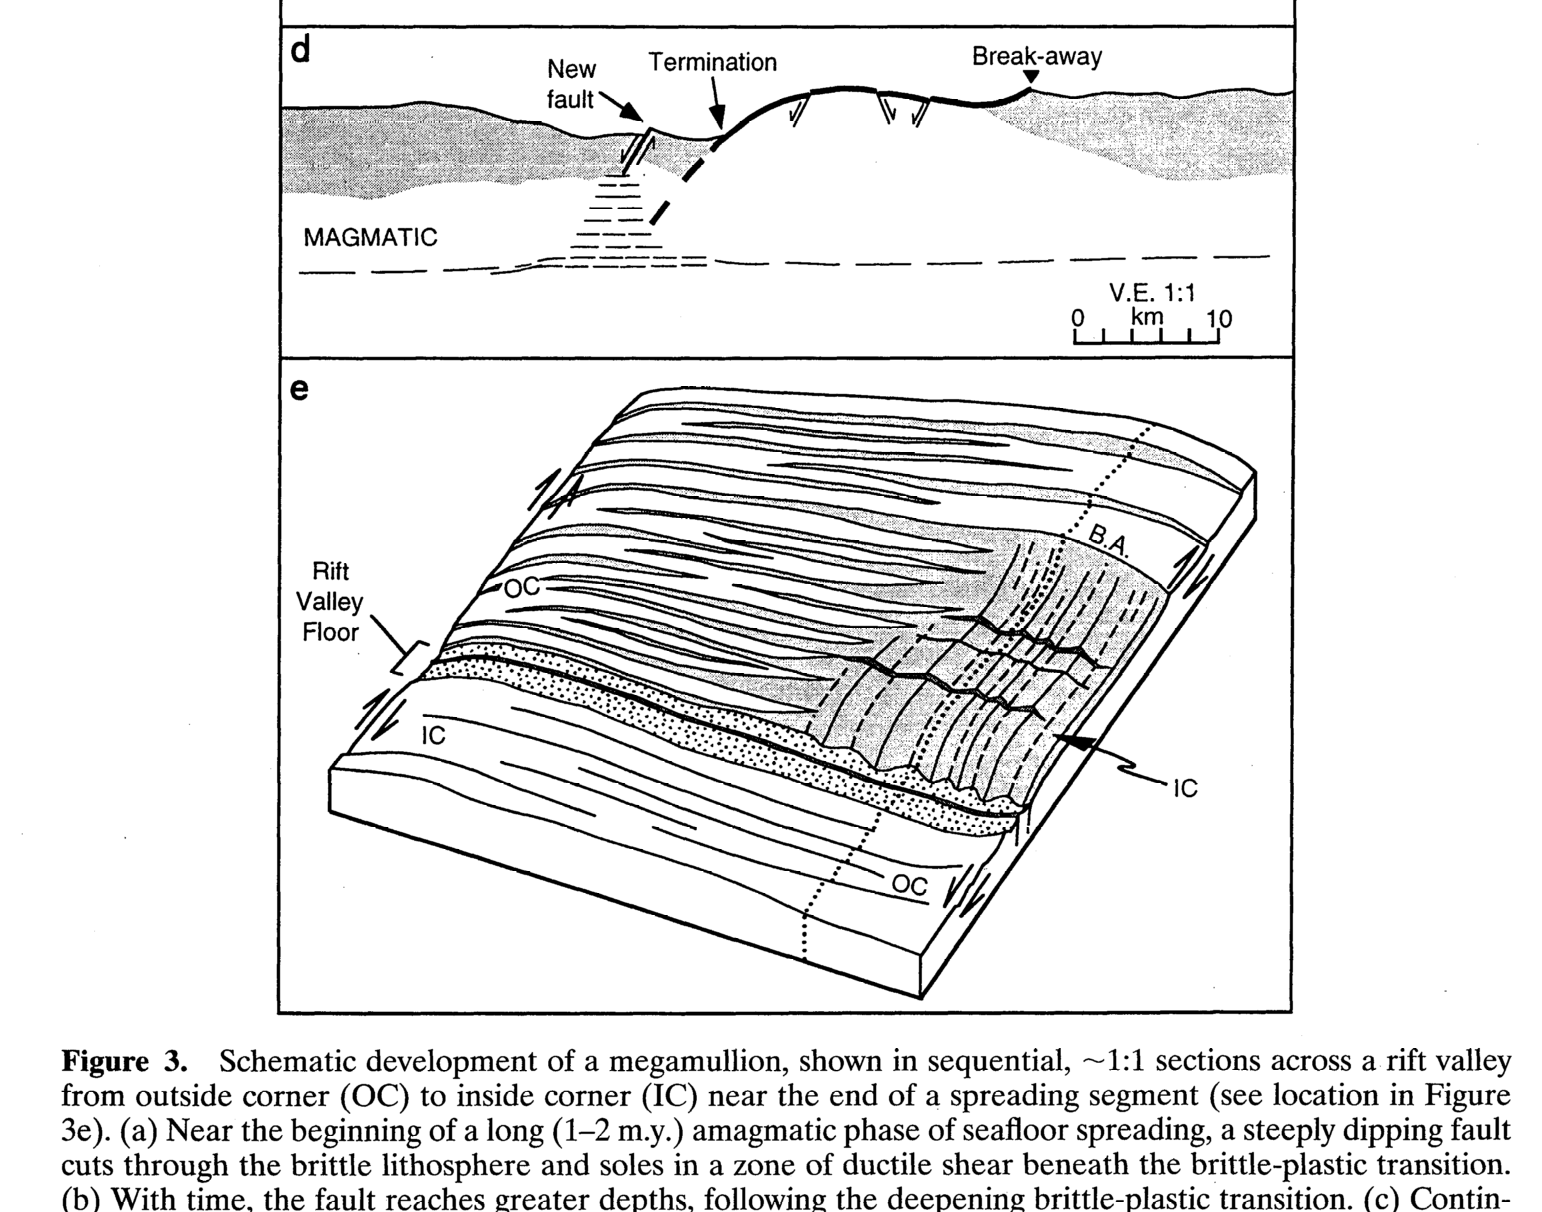
\includegraphics[width=.9\linewidth]{./fig1_high_angle_fault_at_OCC_surface.png}
\add[XT]{the high angle shallow fault cut the surface of OCC can be related to the cut back behavior in the model. Caused by bending stresses during footwall rollover }

Both continental and oceanic core complexes appear to expose deep plastically deformed rocks that \add[Q]{experienced increasingly brittle deformation and retrograde metamorphism as they were exhumed[Hodges 1987; Jaroslow 1996].}

\begin{enumerate}
\item {\bfseries\sffamily TODO} Study \add[Q]{Hess Deep}.
\label{sec-1-2-5-1}
\end{enumerate}

\subsection{6. Dick, H. J. B. et al. A long in situ section of the lower ocean crust: Results of ODP Leg 176 drilling at the Southwest Indian Ridge. Earth Planet. Sci. Lett. 179, 31–51 (2000).}
\label{sec-1-3}
\subsection{7. Blackman, D. K. et al. Geology of the Atlantis Massif (Mid-Atlantic Ridge, 30◦ N): Implications for the evolution of an ultramafic oceanic core complex. Mar. Geophys. Res. 23, 443–469 (2002).}
\label{sec-1-4}
\subsection{8. MacLeod, C. J. et al. Direct geological evidence for oceanic detachment faulting: The Mid-Atlantic Ridge, 15◦450 N. Geology 30, 879–882 (2002).}
\label{sec-1-5}
\subsection{9. Dick, H. J. B., Tivey, M. A. \& Tucholke, B. E. Plutonic foundation of a slow-spreading ridge segment: Oceanic core complex at Kane Megamullion, 23◦300 N, 45◦200 W. Geochem. Geophys. Geosyst. 9, Q05014 (2008).}
\label{sec-1-6}
\subsection{10. MacLeod, C. J. et al. Life cycle of oceanic core complexes. Earth Planet. Sci. Lett. 287, 333–344 (2009).}
\label{sec-1-7}
\subsection{11. Xu, M., Canales, J. P., Tucholke, B. E. \& DuBois, D. L. Heterogeneous seismic velocity structure of the upper lithosphere at Kane oceanic core complex, Mid-Atlantic Ridge. Geochem. Geophys. Geosyst. 10, Q10001 (2009).}
\label{sec-1-8}
% Emacs 24.4.1 (Org mode 8.2.10)
\end{document}
